\chapter{Literature review}
\label{sec_lit_study}
This dissertation deals primarily with stochastic model predictive control but applied within the context of probabilistic graphical models. In Section \ref{sec_stoch_mpc_lit} we briefly discuss some recent developments in stochastic model predictive control literature. In Section \ref{sec_switch_mpc_lit} we briefly discuss control schemes, primarily  based on model predictive control, where the model control is based upon is automatically adjusted based on plant measurements or manual control laws.

\section{Stochastic model predictive control}
\label{sec_stoch_mpc_lit}
Linear unconstrained stochastic control subject to white additive Gaussian noise is well studied in literature. The solution of the linear quadratic gaussian (LQG) controller, for which the problem is shown in (\ref{eq_lit_lqg}), is one of the most fundamental results in stochastic optimal control theory \cite{lqg}. Please note, for stochastic processes it is customary to denote the current time step $x_t$ by $x_0$ within the control optimisation problem. Also, $x_t$ is a latent variable observable only through $y_t \sim \mathcal{N}(Cx_t, V)$. We use boldface to denote a vector of vectors over time e.g. $\mathbf{u}=(u_0, u_1,...)$.
\begin{equation}
\begin{aligned}
&\underset{\mathbf{u}}{\text{min }} V(x_0, \mathbf{u}) = \mathbb{E}\left[ \frac{1}{2}\sum_{k=0}^{N-1} \left( x_k^TQx_k + u_k^TRu_k \right) + \frac{1}{2}x_N^TP_fx_N \right] \\
& \text{subject to } x_{t+1}=Ax_t+Bu_t + w_t~\text{with } w_t \sim \mathcal{N}(0, W) \\
\end{aligned}
\label{eq_lit_lqg}
\end{equation}
Using stochastic Dynamic Programming it is possible to show that the solution of (\ref{eq_lit_lqg}) is merely the solution of the corresponding fully observed deterministic system, called the linear quadratic regulator (LQR), given the mean of the current state estimate $x_0$. A significant drawback of the LQG controller, and by extension the LQR controller, is that it is inherently linear and unconstrained.

Conventional deterministic MPC is very well studied in literature \cite{raw} and can be seen as the constrained deterministic generalisation of the LQG controller as shown in (\ref{eq_lit_mpc}) for one constraint with prediction and control horizon length $N$. The multiple constraint generalisation is straightforward.
\begin{equation}
\begin{aligned}
&\underset{\mathbf{u}}{\text{min }} V(x_0, \mathbf{u}) = \frac{1}{2}\sum_{k=0}^{N-1} \left( x_k^TQx_k + u_k^TRu_k \right) + \frac{1}{2}x_N^TP_fx_N \\
& \text{subject to } x_{t+1} = Ax_t+Bu_t \\
& \text{and } d^Tx_t + e \geq 0 ~\forall~t=1, 2,...,N \\
\end{aligned}
\label{eq_lit_mpc}
\end{equation}
A further generalisation of deterministic MPC is stochastic MPC whereby either the variables, the constraints or both have stochastic elements. In current literature the trend is to convert all the stochastic elements of the control problem into deterministic ones. This usually makes the problem somewhat more tractable from an analytic and computational point of view.

This conversion is usually achieved via two distinct approaches. In the first approach, which is also the one we employ, the probability distributions are assumed Gaussian and the systems linear. This allows one to greatly simplify the problem at the cost of those relatively strong assumptions. The second approach is to use a particle/sampling approach. Here the probability distributions are approximated by particles/samples and no assumptions are made of form of the distributions. It is also not necessary to assume linear dynamics. The major practical drawback of this approach is that it can quickly become computationally intractable for large problems.

Indeed, this is the approach taken by \cite{blackmore}. They attempt to solve the stochastic MPC problem shown in (\ref{eq_lit_chance_mpc_state}) with stochastic (chance) constraints and variables by approximating the current and predicted distributions with particles. Note that $w_t$ is some stochastic variable with known parametrisation.
\begin{equation}
\begin{aligned}
&\underset{\mathbf{u}}{\text{min }} \mathbb{E}\left[ \frac{1}{2}\sum_{k=0}^{N-1} \left( x_k^TQx_k + u_k^TRu_k \right) + \frac{1}{2}x_N^TP_fx_N \right] \\
& \text{subject to } x_{t+1}=Ax_t+Bu_t + w_t \\
& \text{and } \mathbb{E}[d^Tx_t + e] \geq 0 ~\forall ~t=1,...,N \\
& \text{and } \text{Pr}(d^Tx_t + e \geq 0) \geq p ~\forall ~t=1,...,N\\
\end{aligned}
\label{eq_lit_chance_mpc_state}
\end{equation}
In their approach a particle filter is used as the state estimator; the current state distribution is approximated by particles of equal weight. An integer variable is then introduced for each particle at each predicted time step. The chance constraint is then enforced by requiring that at least a certain number of particles satisfy the constraint. It is not clearly stated but this approach is only valid for particles after re-sampling. 

By using the particle approach to model distributions it is possible to convert the stochastic optimisation problem into a deterministic one. In the case where linear dynamics are used this becomes a mixed integer linear or quadratic programming problem depending on the objective function. The chance constraint becomes an integer constraint. Their algorithm is appealing because it is not necessary to assume Gaussian distributions or linearity. However, it is possible that the algorithm can become computationally intractable due to the integer constraints which are used to approximate the chance constraints. Since it is necessary to include an integer variable for each particle at each time step in the prediction horizon the number of variables can become large. For large problems with long prediction horizons this can be problematic.  

The approach taken by \cite{li} is related to the sampling approach. They convert the stochastic chance constrained optimisation problem into a deterministic nonlinear optimisation problem. They then use a simulation approach to ensure that the chance constraints are satisfied. Their approach is numerically intensive due to the sampling and gradient estimation techniques. The approach taken by \cite{batina} uses a randomized optimisation algorithm in concert with the empirical mean of the variables. When the states approach a constraint a penalty method is used to heavily penalise the system to steer it away from the constraint. This causes the system to conservatively satisfy the constraints.

In \cite{li2} the stochastic variables are assumed to be Gaussian and the stochastic optimisation problem is transformed into a nonlinear optimisation problem. Using the Gaussian assumption they are able to ensure feasibility and constraint satisfaction albeit conservatively. In \cite{masahiro} the feasibility of stochastically constrained predictive control is considered. Feasibility becomes a problem when predicting under uncertainty. Since the current state estimate is not precisely known and the evolution of the system is stochastic, the certainty of the predicted states often decreases with the prediction horizon. Ensuring constraint satisfaction can become problematic in such situations because of the large predicted uncertainty in the future. In \cite{masahiro} an algorithm enforcing joint chance constraints and recursive feasibility is discussed using a risk allocation approach. While \cite{schwarm} mainly concerns stochastic parameters in the optimisation problem it is shown that chance constraints can, in theory, be rewritten as deterministic constraints if the probability distributions are known and affine constraints are used. 

In \cite{vanhessem2} and \cite{vanhessem1} an ellipsoidal approximation technique is used to ensure constraint satisfaction for the problem shown in (\ref{eq_lit_chance_mpc_vanhessem}). The authors use the expected value of the stochastic variables in the objective function and system dynamics. They also only consider deterministic linear objective functions. The randomness introduced by the stochastic variables is only addressed in the chance constraint. 
\begin{equation}
\begin{aligned}
&\underset{\mathbf{u}}{\text{min }} f(\mathbf{x}) \\
& \text{subject to } x_{t+1}=Ax_t+Bu_t \\
& \text{and } \text{Pr}(d^Tx_t + e \geq 0) \geq p ~\forall ~t=1,...,N\\
\end{aligned}
\label{eq_lit_chance_mpc_vanhessem}
\end{equation}
If one assumes that each $x_t$ is Gaussian with sufficient statistics $(\mu_t, \Sigma_t)$ and dimension $n$, then the chance constraint can be satisfied by ensuring that the area of each ellipse $(x-\mu_t)^T\Sigma_t^{-1}(x-\mu_t)=k^2$ for $t=1,...,N$ is contained in the feasible region. We have that $k^2$ is chosen by solving the integral equation of the Chi Squared distribution as shown in (\ref{eq_lit_chi_squared}).
\begin{equation}
\frac{1}{2^{\frac{n}{2}}\Gamma(\frac{n}{2})}\int_0^{k^2}\mathcal{X}^{\frac{n}{2}-1}e^{-\frac{\mathcal{X}}{2}}d\mathcal{X} = p
\label{eq_lit_chi_squared}
\end{equation} 
Using the ellipsoidal approximations the stochastic optimisation problem can transformed into a second order conic optimisation problem. The authors ensure that each ellipse is contained in the feasible region by ensuring there exists sufficient ``back-off" (the distances $z_1$, $z_2$, $z_3$ and $z_4$) between the predicted ellipses and the constraints as shown in Figure \ref{fig_vanhessem}.
\begin{figure}[H]
\centering
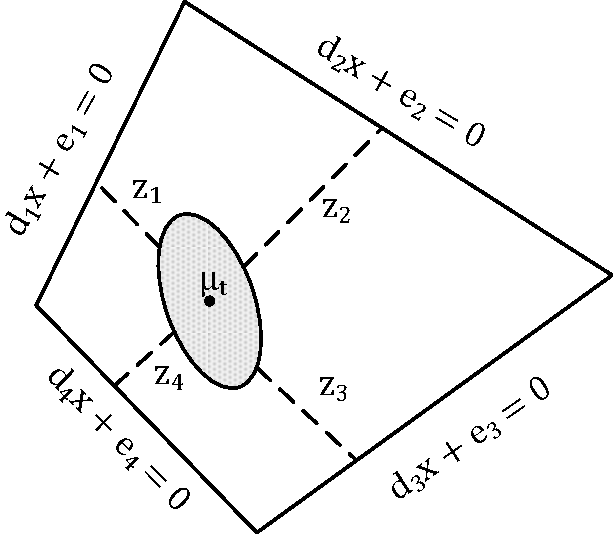
\includegraphics[scale=0.8]{vanhess.pdf}
\caption{Ellipsoidal approximation to ensure chance constraint satisfaction as used by \cite{vanhessem2} and \cite{vanhessem1}.}
\label{fig_vanhessem}
\end{figure}
While this breakthrough is important - we build on it in our approach - the authors do not realise that they are in fact using a form of the Mahalanobis distance to enforce their chance constraints. The approach of using confidence ellipsoids is further refined in \cite{cannon}. The ellipsoidal approximation technique is also further investigated in \cite{blackmore2}; they show that is is possible to reformulate joint chance constraints using univariate Gaussian distributions.

Although \cite{yan1} and \cite{yan2} primarily deal with univariate problems they show that if the underlying system is linear and Gaussian, it is possible to manipulate the constrained stochastic problem shown in (\ref{eq_lit_chance_mpc_state}) into a deterministic problem. Their analysis allows the stochastic objective function to be transformed into its deterministic equivalent using the properties of Gaussian integrals. This development is quite important because it allows one to directly evaluate the stochastic objective function. The constraints are handled by directly evaluating the Gaussian integral corresponding to the chance constraint in the univariate case. The authors allude to the fact that this becomes computationally intractable in higher dimensions and suggest that the approach in \cite{vanhessem2} be used. The authors also suggest a way to handle the situation where covariance matrix grows without bound in unstable systems. This is related to the feasibility problems discussed earlier.

In this dissertation we illustrate the benefits gained by designing controllers within the framework of probabilistic graphical models. We investigate and show the following:
\begin{enumerate}
\item
Under the assumption of normality and linearity it is possible to convert the stochastic objective function of (\ref{eq_lit_lqg}) into its deterministic equivalent. The analysis is closely related to the work of  \cite{yan1} and \cite{yan2} but we show that these results are immediately obvious from within the framework of probabilistic graphical models. Thus it is possible to solve the LQG problem without resorting to stochastic dynamic programming.
\item
We generalise our analysis to stochastic MPC and show that by using the statistically important metric, the Mahalanobis distance, we arrive at a technique for enforcing chance constraints which is very closely related to the approach by \cite{vanhessem2} and \cite{vanhessem1}. Under the assumption of linearity and normality we show that the constraint satisfaction is ensured. Due to the use of the Mahalanobis Distance metric we provide some theoretical support for the use of the ``ellipsoidal approximation" technique if the underlying system is non-linear or not exactly Gaussian.
\item
Combining the previous results we show that it is possible to write the joint chance constrained stochastic MPC problem as a deterministic MPC problem. Additionally we show that the joint chance constraints can be written in a linear format. The entire optimisation problem can then be written in the standard form for auadratic programming optimisation. Standard deterministic MPC solution techniques can then be used to solve the stochastic problem.
\item
We compare the effect different inference techniques have on the quality of the MPC.
\end{enumerate}
Lastly, measurement and system noise is ubiquitous in real life systems. Therefore most modern model predictive control systems use an inference (filtering) technique to estimate the current system state. By using a filter the control system is implicitly using a probabilistic graphical model; therefore we are not actually introducing anything exotic but rather highlighting a connection between two rich fields. 

\section{Switching model predictive control}
\label{sec_switch_mpc_lit}
In model predictive control the model of the plant is used to predict the future behaviour of the plant given some inputs which are optimised according to some performance criterion. Classically this model is linear and time invariant. An example of such a model is shown in (\ref{eq_mpc_nodisturbance_obs}); since it includes system and measurement noise a state estimator would typically be used to infer $x_t$. The mean of the current state, $\mathbb{E}[x_t]$ together with the deterministic state model $x_{t+1} = Ax_t + Bu_t$ would then be used for prediction \cite{raw}. This assumption allows for the use of advanced constrained optimisation algorithms, typically Quadratic Programming algorithms. From a practical perspective robust and fast optimisation is crucial because it allows control inputs to be calculated on-line \cite{mac}.
\begin{equation}
\begin{aligned}
&x_{t+1} = Ax_t + Bu_t + w_t~\text{(Latent)} \\
&y_t = Cx_t + v_t~\text{(Observed)}
\end{aligned}
\label{eq_mpc_nodisturbance_obs}
\end{equation}
Unfortunately modelling errors or omissions often cause poor controller performance within the context of MPC. This is often observed as steady state offset i.e. the controller takes no more action and the system is not at the set point. In certain cases it is possible to account for plant/model mismatch or asymptotically constant disturbances by incorporating a disturbance model within the MPC framework. This is classically called zero offset regulation \cite{raw} and is achieved by augmenting the system models as shown in (\ref{eq_mpc_disturbance_obs}).
\begin{equation}
\begin{aligned}
&x_{t+1} = Ax_t + Bu_t + B_d d_t + w_t~\text{(Latent)} \\
&d_{t+1} = d_t ~\text{(Latent)}\\
&y_t = Cx_t + C_d d_t + v_t~\text{(Observed)}
\end{aligned}
\label{eq_mpc_disturbance_obs}
\end{equation}
By using a state estimator the integrating disturbance $d_t$ can be estimated. The model used for prediction is then augmented to incorporate this disturbance $x_{t+1} = Ax_t + Bu_t + \mathbb{E}[d_t]$ \cite{lee}. The problem with this approach is that it assumes that the model $(A, B)$ is at least somewhat representative of the underlying dynamics.

Linear models $(A, B)$ are often derived by linearising non-linear models about a single operating point. These models are traditionally used in MPC design; a drawback with this approach is that linear models are fundamentally only accurate in a small region around the point of linearisation. The further the system moves away from the linearisation point the worse the accuracy of the model becomes because the model is no longer a good approximation of the underlying system dynamics. A possible solution to this problem is Non-linear MPC (NMPC). In NMPC the full non-linear model is used for controller design; it is hoped that this more complicated model is accurate over the entire problem domain. Unfortunately this approach is often computationally intensive, especially for large problems, because it inherently requires non-linear, usually non-convex, optimisation. This is a subject of much current research \cite{diehl}. 

Another approach is to approximate a potentially complex non-linear system by a set of linear functions which are valid in certain ranges. An early attempt at this idea \cite{bemporad} integrated logical rules for switching between different system dynamics and constraints. Using that approach a set of logical rules were integrated into the optimisation problem to yield, in the setting of standard MPC, a Mixed Integer Quadratic Program (MIQP) with linear constraints. This approach is called Mixed Logical Dynamical Modelling (MLD) in literature; the system dynamics are then specified by (\ref{eq_mld_system}) where $i=1,2,..., I$ are the indices of the models approximating the underlying problem.
\begin{equation}
\begin{aligned}
&x_{t+1} = \sum_{i=1}^I \delta_i A_i x_t + \sum_{i=1}^I \delta_i B_i u_t \\
&y_t = \sum_{i=1}^I \delta_i C_i x_t 
\end{aligned}
\label{eq_mld_system}
\end{equation}
The binary variable $\delta_i \in [0, 1]$ selects which linear model to use at each step in the prediction horizon within the framework of MPC. Constraints on $\delta_i$ allow the optimisation algorithm to switch between models based on its position in the state space.  The drawbacks with this approach is that the ``IF-THEN-ELSE" rules need to be fully specified and MIQP can become computationally intractable. 

The work by \cite{du} and \cite{sakakura} elaborate on this approach. Both papers deal with the control of Continuously Stirred Tank Reactors (CSTRs) throughout different operating regimes. CSTRs are a good case study because they often have multiple steady states, constraints and can be quite non-linear. The approach of \cite{du} and \cite{sakakura} is to linearise the underlying non-linear CSTR model about different operating points and use those models to approximate the true non-linear dynamics. Computational difficulties are reported because the complexity of the MIQP problem scales exponentially with the number of variables.

The approach by \cite{ozkan} is similar except that they use ellipsoidal regions to develop a multiple model MPC. Again the approach by \cite{kvasnica} is similar except that they attempt to reduce the complexity of the MIQP problem by providing guidelines on selecting the number of linear models used. More linear models leads to better control but the optimisation problem becomes correspondingly more difficult. Finally, \cite {nandola} also investigates hybrid systems but uses Bayes' Theorem to assign weights to the different models as opposed to only having one model active in each region. In their approach $\delta_i$ is a continuous variable in the range $[0, 1]$ and $\sum_{i=1}^I \delta_i = 1$. While their approach is also computationally intensive, a mixed integer non-linear optimisation problem needs to be solved, an effort is made to take advantage of the problem structure to attenuate this problem.

Loosely related to the idea of model switching is model based fault detection. In \cite{isermann} it is found that almost 70\% of the reviewed papers dealing with fault detection use observer or parameter estimation methods. The basic idea behind this approach is to estimate the system outputs using an observer and to compare this to some model of the system. The difference, often called the residual, is then used to estimate the probability of a fault in the process \cite{edwards}. The approach followed in \cite{wang} combines elements of model switching and state observations. They use a filter to construct a residual generator which is used to evaluate whether or not the system has a fault. The filter can switch between the different linear system models based on the current regime of the system. 

Related to this class of model based fault detection algorithms is the Switching Particle Filter or Switching Kalman Filter if the underlying system is linear and Gaussian. The corresponding Probabilistic Graphical Model is shown in Figure \ref{fig_spf_skf}.
\begin{figure}[H] 
\centering
\begin{tikzpicture}

  % Define nodes
  \node[obs] (ya) {$y_0$};
  \node[obs, right=of ya] (yb) {$y_1$};
  \node[obs, right=of yb] (yc) {$y_2$};
  \node[latent, above=of ya]  (xa) {$x_0$};
  \node[latent, above=of yb, right=of xa]  (xb) {$x_1$};
  \node[latent, above=of yc, right=of xb]  (xc) {$x_2$};
  \node[latent, above=of xa] (sa) {$s_0$};
  \node[latent, above=of xb] (sb) {$s_1$};
  \node[latent, above=of xc] (sc) {$s_2$};
  
  % Connect the nodes
  \edge {xa} {ya};
  \edge {xb} {yb};
  \edge {xc} {yc};
  \edge {xa} {xb};
  \edge {xb} {xc};
  \edge {sa} {sb};
  \edge {sb} {sc};
  \edge {sa} {xa};
  \edge {sb} {xb};
  \edge {sc} {xc};
  
\end{tikzpicture}
\caption{Switching Filter Graphical Model}
\label{fig_spf_skf}
\end{figure}
Classically these types of models are used to infer the current state  estimate (called filtering) given a set of models. Intuitively, the model which best describes the current observation ($y_t$) is assigned the most weight in the state estimate. This allows for the modelling of non-linear and multi-modal distributions by combining models based on the inferred switching variable ($s$) \cite{murphy1}. These models may be used for both filtering and event detection (see \cite{veerar} for an example) which, in the setting of control, can be interpreted as fault detection.

In this dissertation we also illustrate the potential benefits gained by designing controllers using non-standard probabilistic graphical models, specifically Figure \ref{fig_spf_skf}. We investigate and show the following:
\begin{enumerate}
\item
Using the Rao-Blackwellised Particle Filter it is possible to accurately estimate the current state using linear models. The state estimate can then be used within the controller framework alluded to in Chapter \ref{sec_stoch_mpc_lit}. Using this approach it is also possible to change the model control is based upon. The linear model which best describes the current observations is used for control purposes. In this way we gain the benefit of model switching but do not incur the significant computational cost when it is incorporated into the optimisation problem. We call this approach the Switching Controller Algorithm.
\item
Using the Switching Particle Filter it is possible to accurately estimate the current state using non-linear models. The same Switching Controller Algorithm is used but implemented using the Switching Particle Filter. In this setting the filter discerns between a healthy and faulty system and uses the best model to effect control.
\item
In both cases the Switching Controller Algorithm is not robust enough against model selection (switching) noise. However, the results indicate that the approach is promising.
\end{enumerate}
Even more so than Chapter \ref{sec_stoch_mpc_lit}, the approach used here relies on the application of probabilistic graphical models to controller design.  



